% Figure 7 -- the three dimensional mirror of the gauge theory of figure 6
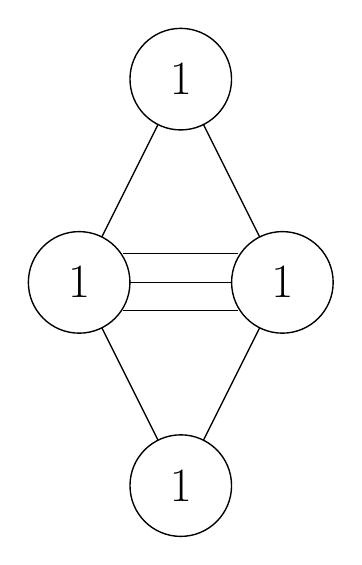
\begin{tikzpicture}[x=1.8pt,y=1.8pt,>=stealth,line width=0.5pt,
    nd/.style={circle,draw,fill=white,inner sep=0pt,minimum size=36.7pt,
               font=\fontsize{16.4}{19}\selectfont}]
  % the two horizontal links between the left and the right node
  \draw (24.4,47.7) -- (47.4,47.7);
  \draw (24.4,59.2) -- (47.4,59.2);
  % the four legs
  \draw (15.5,53.4) -- (35.9,94.2);
  \draw (35.9,94.2) -- (56.3,53.4);
  \draw (15.5,53.4) -- (35.9,12.6);
  \draw (35.9,12.6) -- (56.3,53.4);
  \draw (25.7,53.4) -- (46.1,53.4);
  % nodes
  \node[nd] at (15.5,53.4) {1};
  \node[nd] at (56.3,53.4) {1};
  \node[nd] at (35.9,94.2) {1};
  \node[nd] at (35.9,12.6) {1};
\end{tikzpicture}
